\section{Introduction}
\label{sec:intro}

The choice of which structures to prune from a reasoning LLM shapes whether the model sustains reinforcement learning alignment.
Current compression pipelines treat this choice as independent of downstream training: structured pruning removes entire attention heads or MLP channels to reduce memory and latency~\citep{llmpruner2023,graspprune2026}, Supervised Fine-Tuning (SFT) recovers task accuracy, and Reinforcement Learning with Verifiable Rewards (RLVR) restores reasoning quality~\citep{deepseek2025r1,shao2024grpo}.
Each stage is optimized in isolation.
We demonstrate that this separation fails: the pruning criterion significantly influences what we term \textbf{recovery capacity}, the model's ability to sustain RL-based recovery without collapsing into degenerate outputs.

The consequences of ignoring this coupling are severe: GRPO training on pruned models can trigger complete collapse, with gradient norms approaching zero, repetitive outputs, and monotonically degrading reward.
Whether collapse occurs depends entirely on which structures were removed.
Reward itself is an unreliable diagnostic: on unpruned DeepSeek-R1-Distill-Qwen-7B~\citep{deepseek2025r1}, 100 steps of Group Relative Policy Optimization (GRPO;~\citealp{shao2024grpo}) raise mean reward from 0 to 0.669 while greedy accuracy on GSM8K~\citep{cobbe2021gsm8k} remains exactly 81.27\%.\footnote{The unpruned model achieves 90.83\% without fine-tuning. Applying the same SFT recovery protocol designed for pruned models reduces accuracy to 81.27\%, consistent with catastrophic forgetting when further fine-tuning an already well-optimized model.}
This reward-accuracy decoupling motivates our focus on recovery capacity as the appropriate diagnostic for post-pruning RL trainability.
\citet{selfhealing2025} claim that RLVR recovers pruned reasoning models to near-original performance, but their evaluation uses a single pruning method and reports only final-checkpoint accuracy without examining training dynamics.

Existing structured pruning methods for reasoning LLMs~\citep{graspprune2026,resp2025,llmpruner2023,bonsai2025,paser2025,pat2025} optimize for post-pruning quality without studying downstream alignment; none compare multiple pruning criteria under RL or study how pruning affects RL training dynamics.
\citet{rlsqueezes2026} show that RL and SFT impose fundamentally different demands on model representations (RL compresses solution paths while SFT expands them), suggesting that pruning decisions should substantially affect RL trainability, yet no prior work has tested this hypothesis.

\begin{figure}[t]
\centering
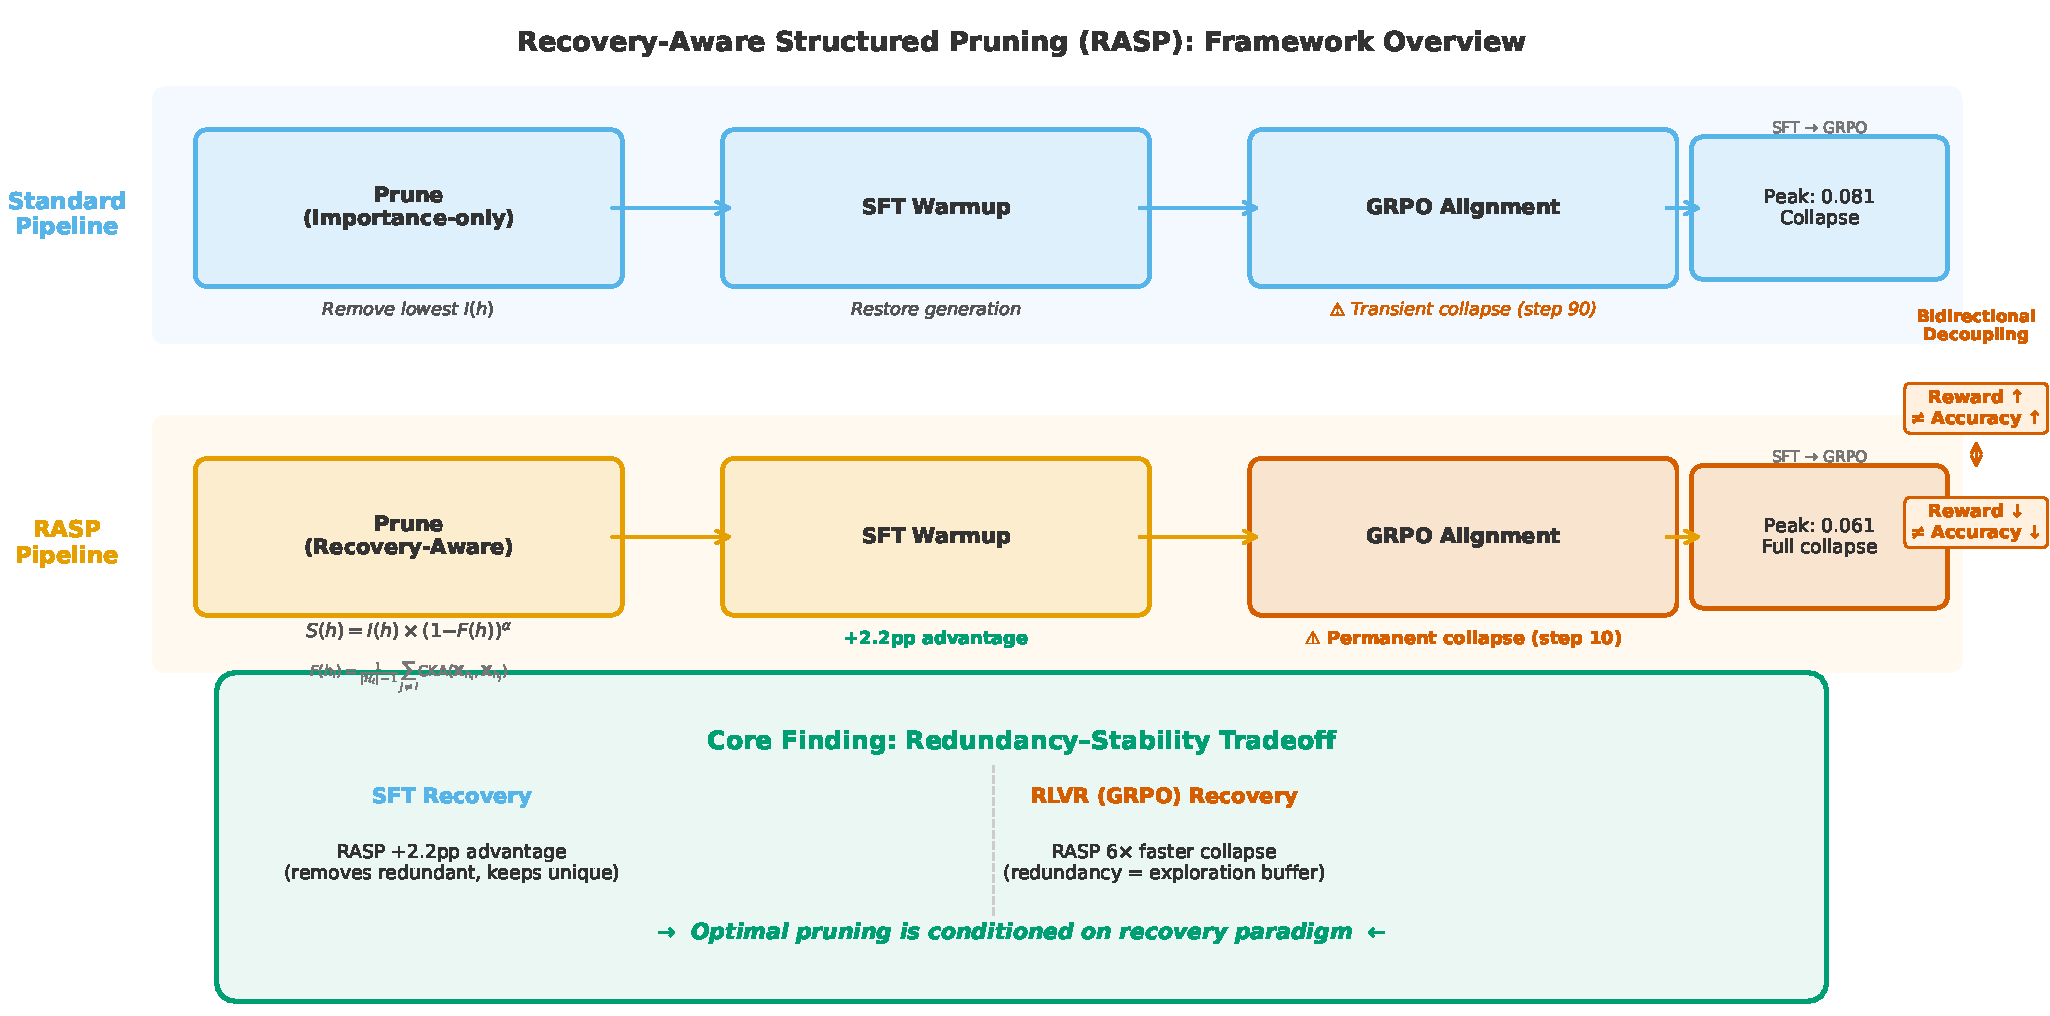
\includegraphics[width=\columnwidth]{../figures/paper/fig1_framework.pdf}
\caption{Controlled comparison framework. All four pruning criteria share the same structural analysis (Taylor importance + CKA overlap) and identical recovery pipeline (SFT warmup $\to$ GRPO). Despite identical training, the criteria produce divergent outcomes: CKA-only achieves active learning while Standard and \rasp{} collapse.}
\label{fig:framework}
\end{figure}

We present a controlled comparison of four structural pruning criteria under identical GRPO training on DeepSeek-R1-Distill-Qwen-7B at 20\% structured sparsity, with cross-architecture validation on Qwen2.5-Math-7B (Figure~\ref{fig:framework}).
The four criteria span a spectrum of representational diversity preservation: \textbf{CKA-only} scoring removes structures with the highest pairwise Centered Kernel Alignment (CKA;~\citealp{kornblith2019cka}) overlap, preserving all representationally unique structures; \textbf{Random} scoring provides an unbiased baseline; \textbf{Standard} importance-only scoring retains structures with the highest gradient-based importance~\citep{llmpruner2023}; and \textbf{Recovery-Aware Structured Pruning} (\rasp{}) combines importance with CKA overlap in a composite score.
Under identical GRPO configuration, these four methods reveal a \textbf{recovery capacity spectrum}.
CKA-only pruning achieves \emph{active learning}: peak reward reaches 0.354 (4.4$\times$ Standard).
Random pruning stagnates (reward oscillates 0.14--0.19).
Standard pruning exhibits borderline collapse (peak 0.081).
\rasp{} collapses permanently (peak 0.061, 85\% of completions yield zero reward variance).
The ordering, CKA-only $\gg$ Random $>$ Standard $>$ \rasp{}, follows the degree of preserved representational diversity.
Gradient importance scoring, the standard criterion for LLM pruning, removes structures scored ``unimportant'' by gradient metrics that are in fact representationally unique, reducing the exploration diversity available for RL training in our setting.
A depth pruning baseline (ShortGPT;~\citealp{shortgpt2024}) is the only method where GRPO actively degrades accuracy ($-$1.36\,pp), confirming that pruning granularity interacts with RL trainability.

Our contributions are:
\begin{enumerate}[nosep,leftmargin=*]
    \item We discover a \textbf{recovery capacity spectrum} across four pruning criteria under controlled GRPO training: CKA-only enables active learning (peak reward 4.4$\times$ Standard), Random stagnates, and Standard/\rasp{} collapse. Extended training (300 steps) confirms this gap is structural. Cross-scale (1.5B) and cross-architecture (Qwen2.5-Math-7B) experiments provide initial evidence for generality (\S\ref{sec:recovery_gradient}, \S\ref{sec:extended_analysis}).
    \item We show that \textbf{reward-accuracy decoupling} is sparsity-dependent: at 15\% sparsity, GRPO amplifies the CKA-only advantage ($+$1.51\,pp differential), while at 20--25\% GRPO cannot improve upon SFT baselines. This motivates reward trajectory as the diagnostic for recovery capacity (\S\ref{sec:decoupling}).
\end{enumerate}
